%%%%%%%%%%%%%%%%%%%%%%%%%%%%%%%%%%%%%%%%%%%%%%%%%%%%%%%%%%%%%%%%%%%%%%%%%%%%%%%%%%
\begin{frame}[fragile]\frametitle{}
\begin{center}
{\Large Game Theory}

{\small {Presh Talwalkar}}


\end{center}
\end{frame}




%%%%%%%%%%%%%%%%%%%%%%%%%%%%%%%%%%%%%%%%%%%%%%%%%%%%%%%%%%%%%%%%%%%%%%%%%%%%%%%%%%
\begin{frame}[fragile]\frametitle{}
\begin{center}
{\Large Game Theory}

{\small Other sources}


\end{center}
\end{frame}



%%%%%%%%%%%%%%%%%%%%%%%%%%%%%%%%%%%%%%%%%%%%%%%%%%%%%%%%%%%
\begin{frame}[fragile]\frametitle{Fair Division}
\begin{columns}
    \begin{column}[T]{0.6\linewidth}
      \begin{itemize}
		\item Problem: While distributing a cake between two brothers, the younger feels that the elder one is cutting into unequal chunks and taking the bigger piece.
		\item Core Issue: Division and Allocation is done by same person.
		\item Solution: Separate both. Meaning, one of them cuts the cake and the other picks. So, almost no chance that the one who divides will make unequal pieces!!
	  \end{itemize}

    \end{column}
    \begin{column}[T]{0.4\linewidth}
		\begin{center}
		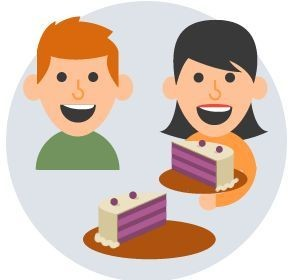
\includegraphics[width=0.8\linewidth,keepaspectratio]{images/game_theory_fair_division}
		
		{\small ``I-Cut-You-Choose'' Cake-Cutting Protocol Inspires Solution to Gerrymandering - 
Byron Spice (SCS) and Jocelyn Duffy (MCS)}
		\end{center}	
    \end{column}
  \end{columns}
\end{frame}














%%%%%%%%%%%%%%%%%%%%%%%%%%%%%%%%%%%%%%%%%%%%%%%%%%%%%%%%%%%
\begin{frame}[fragile]\frametitle{}
\begin{itemize}
\item 
\end{itemize}
\end{frame}

%%%%%%%%%%%%%%%%%%%%%%%%%%%%%%%%%%%%%%%%%%%%%%%%%%%%%%%%%%%
\begin{frame}[fragile]\frametitle{Sample Picture Inclusion}

% \begin{center}
% \includegraphics[width=0.8\linewidth,keepaspectratio]{myphoto}
% \end{center}	  
\end{frame}


%%%%%%%%%%%%%%%%%%%%%%%%%%%%%%%%%%%%%%%%%%%%%%%%%%%%%%%%%%%
\begin{frame}[fragile]\frametitle{Sample Two Columns Slide}
\begin{columns}
    \begin{column}[T]{0.6\linewidth}
      \begin{itemize}
		\item aaa
	  \end{itemize}

    \end{column}
    \begin{column}[T]{0.4\linewidth}
      \begin{itemize}
		\item bbb
	  \end{itemize}
    \end{column}
  \end{columns}
\end{frame}

%%%%%%%%%%%%%%%%%%%%%%%%%%%%%%%%%%%%%%%%%%%%%%%%%%%%%%%%%%%%%%%%%%%%%%%%%%%
\begin{frame}[fragile]\frametitle{References}
\begin{itemize}
\item Farnam Street, Mendtal Models https://fs.blog/mental-models/

\item Farnam Street, How To Deciside: https://fs.blog/smart-decisions/\#how\_to\_decide
\end{itemize}
\end{frame}